\chapter{Конструкторская часть}

В данном разделе будут представлены схемы алгоритмов: полного перебора и муравьиного алгоритма. Будут описаны типы и структуры данных, используемые для реализации, а также структура разрабатываемого программного обеспечения. Кроме того, будут выделены классы эквивалентности для тестирования.

\section{Разработка алгоритмов}

На рисунке \ref{img:brute} приведена схема алгоритма решения задачи коммивояжера полным перебором. Схемы муравьиного алгоритма приведена на рисунке \ref{img:ant}, вспомогательные функции данного алгоритма показаны на рисунках \ref{img:probability}-\ref{img:update}.

\begin{figure}[H]
	\begin{center}
		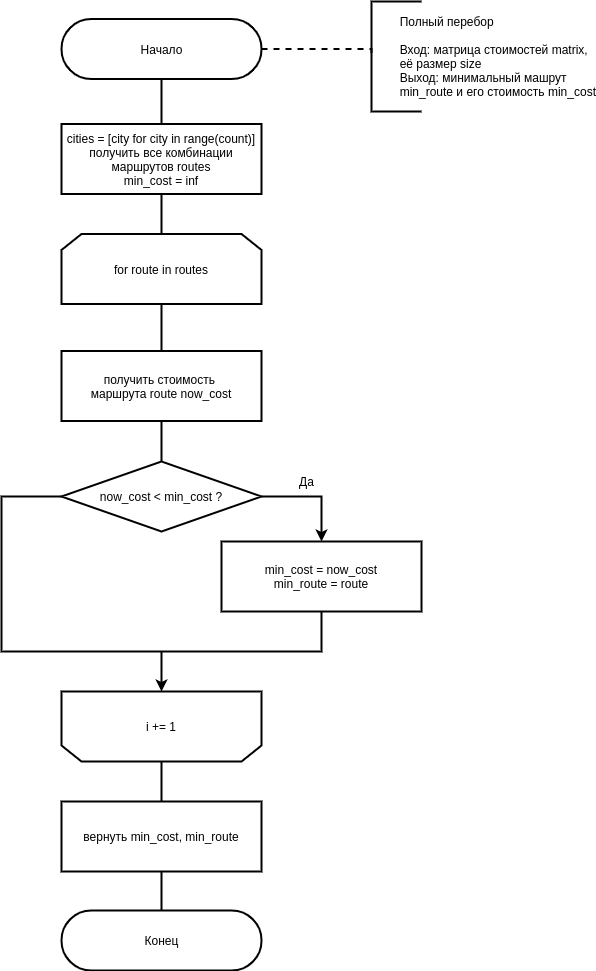
\includegraphics[scale=0.6]{img/brute.png}
	\end{center}
	\captionsetup{justification=centering}
	\caption{Полный перебор}
	\label{img:brute}
\end{figure}

\begin{figure}[H]
	\begin{center}
		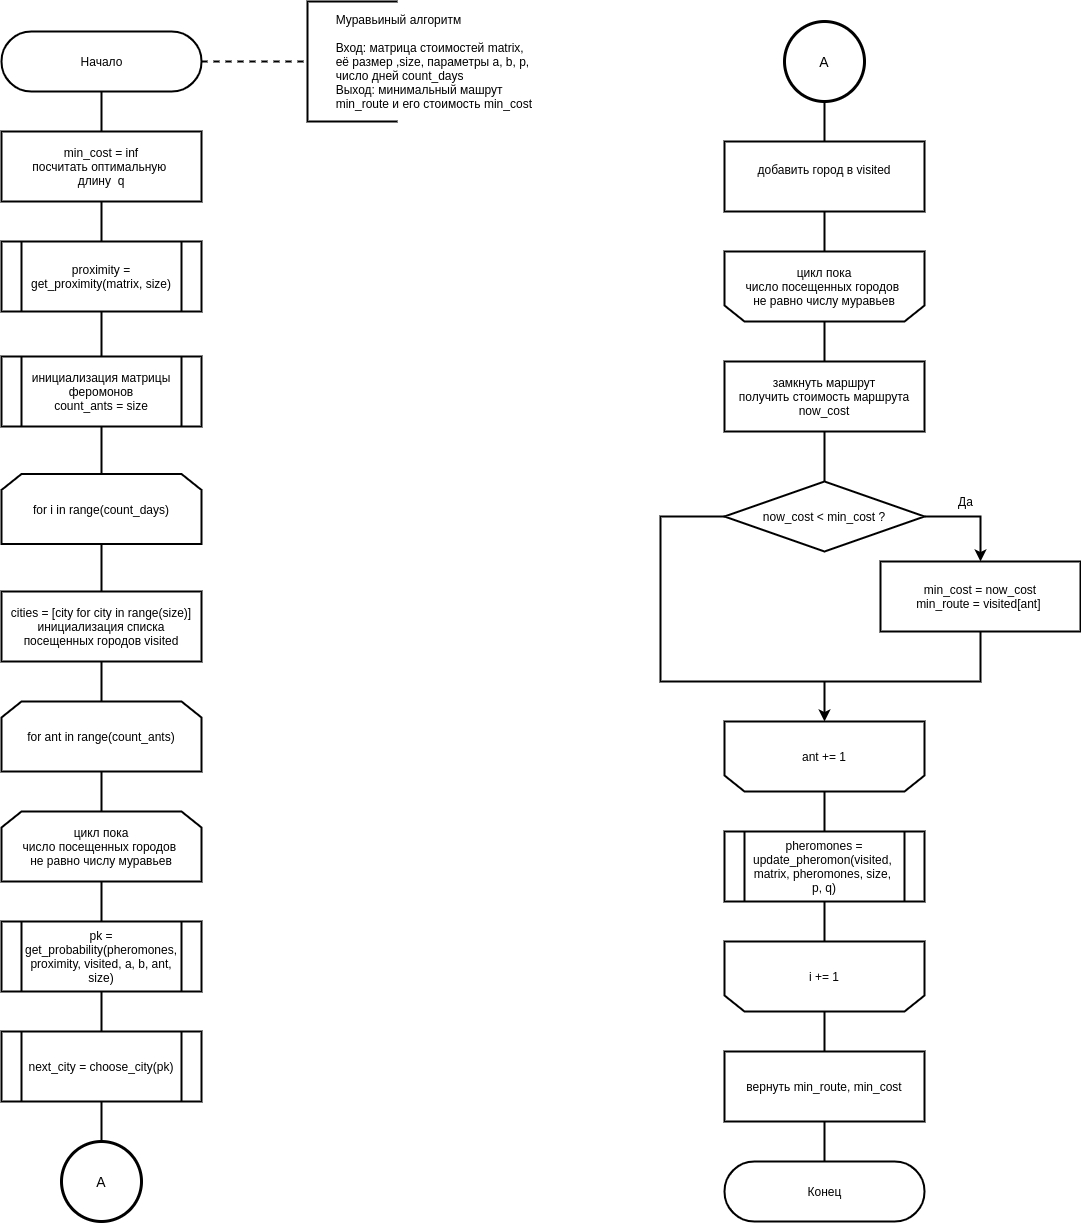
\includegraphics[scale=0.4]{img/ant.png}
	\end{center}
	\captionsetup{justification=centering}
	\caption{Муравьиный алгоритм}
	\label{img:ant}
\end{figure}

\begin{figure}[H]
	\begin{center}
		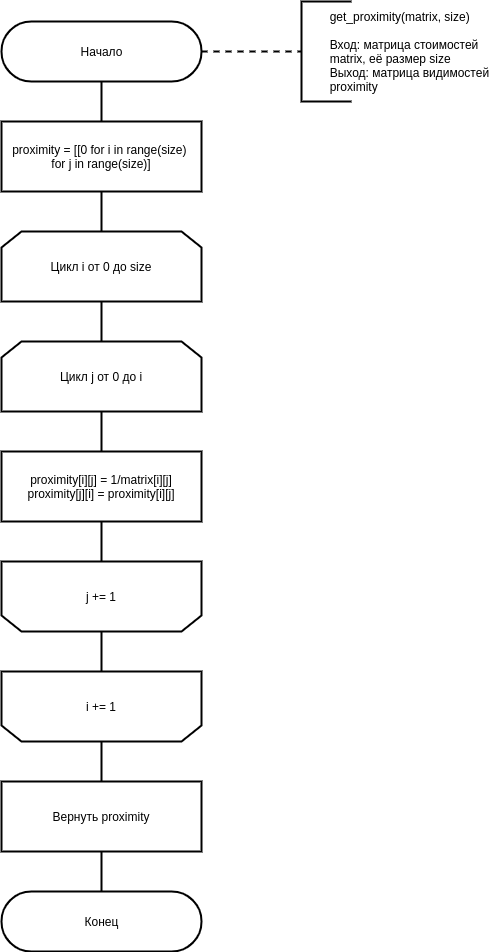
\includegraphics[scale=0.5]{img/proximity.png}
	\end{center}
	\captionsetup{justification=centering}
	\caption{Алгоритм вычисления матрицы видимостей}
	\label{img:proximity}
\end{figure}

\begin{figure}[H]
	\begin{center}
		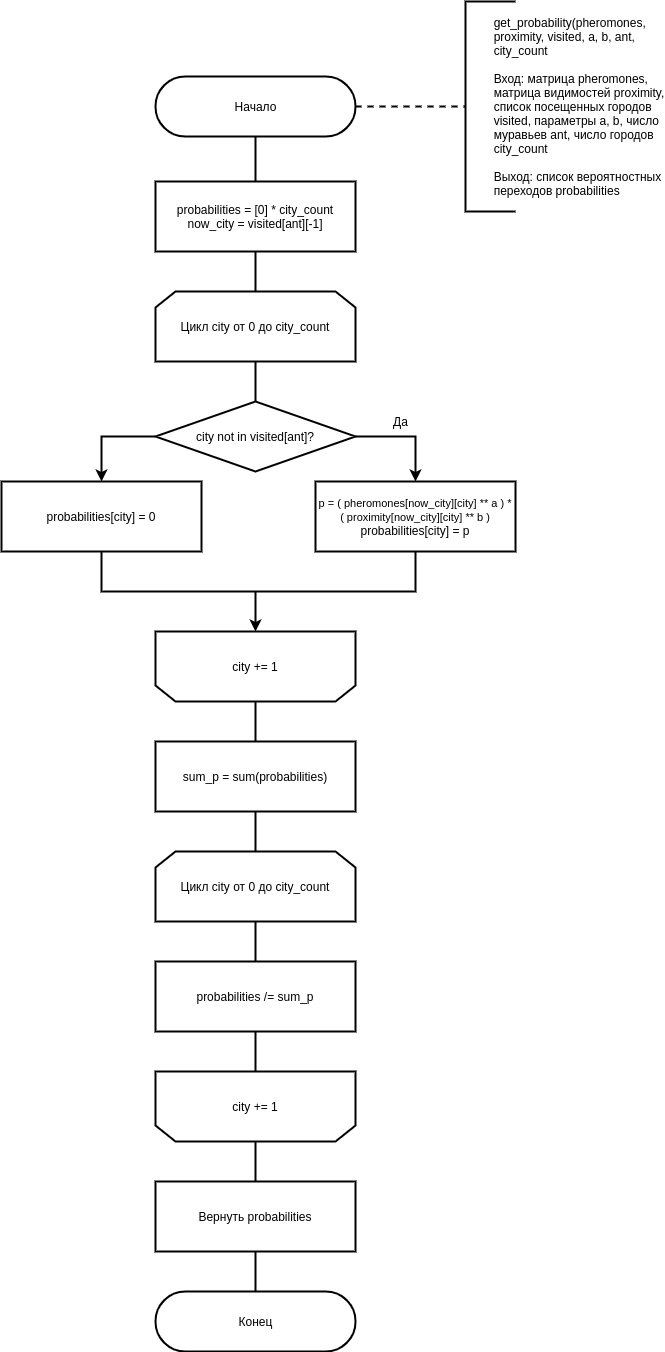
\includegraphics[scale=0.5]{img/probability.png}
	\end{center}
	\captionsetup{justification=centering}
	\caption{Алгоритм вычисления списка вероятностных переходов}
	\label{img:probability}
\end{figure}

\begin{figure}[H]
	\begin{center}
		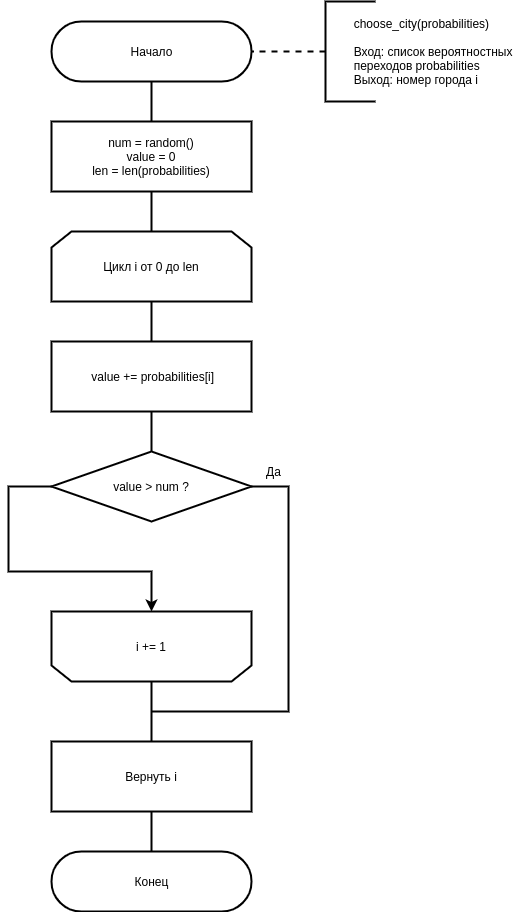
\includegraphics[scale=0.7]{img/choose.png}
	\end{center}
	\captionsetup{justification=centering}
	\caption{Алгоритм выбора следующего города случайным образом}
	\label{img:choose}
\end{figure}

\begin{figure}[H]
	\begin{center}
		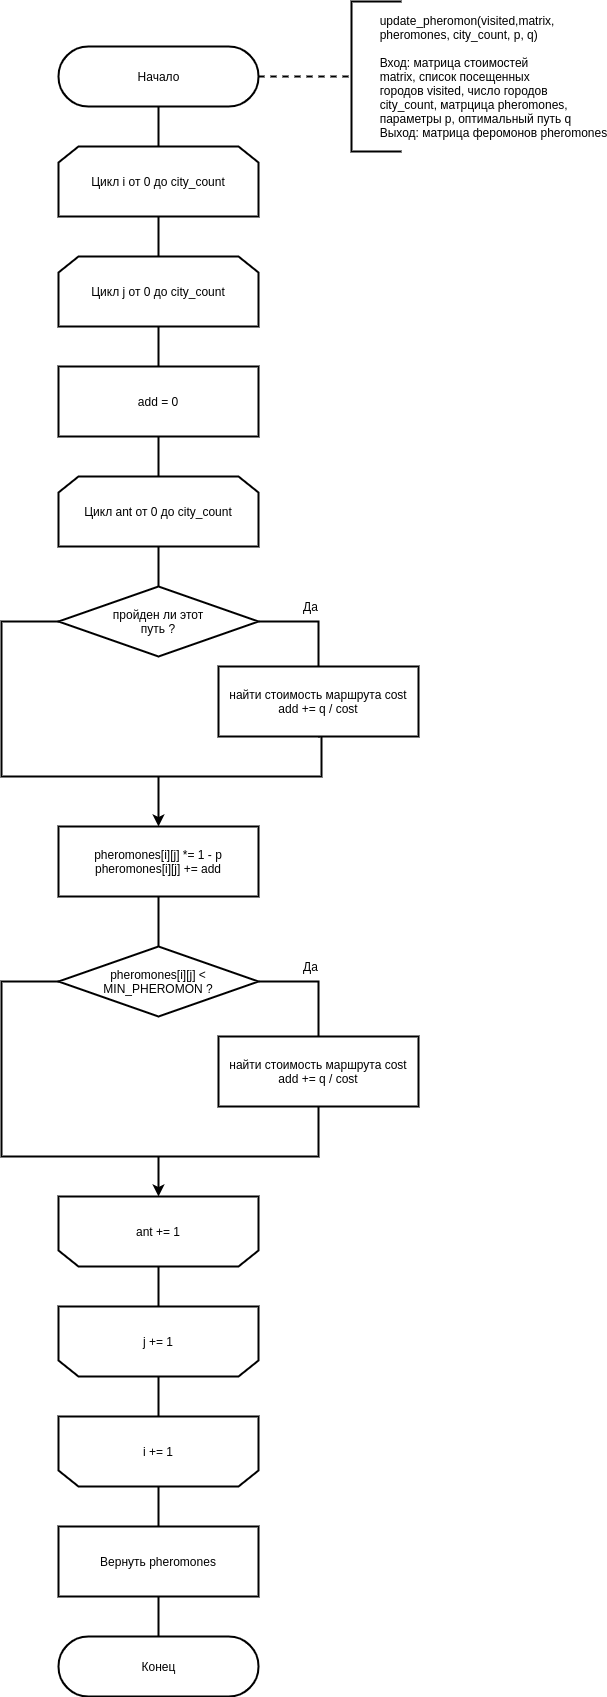
\includegraphics[scale=0.4]{img/update.png}
	\end{center}
	\captionsetup{justification=centering}
	\caption{Алгоритм обновления феромона}
	\label{img:update}
\end{figure}

\section{Описание используемых типов и структур данных}

Для задания числа городов и количества дней поиска будет использован тип данных $int$, для задания параметров $\alpha$, $\beta$ и коэффициента $\rho$ - тип данных $float$.

Структура данных - матрица - представляет собой двумерный список значений типа $int$.


\section{Структура разрабатываемого ПО}

При реализации разрабатываемого программного обеспечения будет использоваться метод структурного программирования. Для взаимодействия с пользователем будет выделена функция $process()$, из которой будут вызываться методы решения задачи коммивояжера, функция параметризации и функции сравнительного анализа. Методы поиска оптимального маршрута будут реализованы в следующих функциях, выходные параметры которых - искомый маршрут и его стоимость:
\begin{itemize}
	\item функция полного перебора маршрутов, у которой на входе - матрица стоимостей и число городов;
	\item функция муравьиного алгоритма, входными параметрами которой являются матрица стоимостей, число городов, параметры $\alpha$, $\beta$, коэффициент $\rho$, число дней поиска.
\end{itemize}

Для работы с матрицей стоимостей будут разработаны следущие функции:

\begin{itemize}
	\item создание матрицы случайных чисел, входным параметром функции является размер, выходным - матрица;
	\item ввод матрицы, входной параметр - размер, выходной параметр - введенная матрица;
	\item процедура вывода матрицы, входным параметром которой является матрица;
	\item чтение матрицы из файла, у функции на входе - имя файла, а на выходе - матрица и ее размер. 
\end{itemize}

Для параметризации будет выделена функция, выходными параметрами которой являются файлы с результатами для двух классов данных.

Для сравнительного анализа будут реализованы:

\begin{itemize}
	\item функция замеров времени, выходным парметром которой является массив временных значений;
	\item функция графического представления замеров времени, у которой на входе - массив временных значений, на выходе - его графическое представление.
\end{itemize}

\section{Классы эквивалентности при тестировании}

Для тестирования разрабатываемой программы будут выделены следующие классы эквивалентности:

\begin{itemize}
	\item неверный ввод параметров $\alpha$, $\beta$, коэффициента $\rho$ и числа дней - не число или число, меньшее или равное 0;
	\item неверный ввод числа дней - не число или число, меньшее 1;
	\item неверный ввод числа городов - не число или число, меньшее 2;
	\item корректный ввод всех параметров.
\end{itemize}

\section{Вывод}

Были представлены схемы поиска оптимального пути, проходящего через все города по одному разу. Были указаны типы и структуры данных, используемые для реализации, и описана структура разрабатываемого программного обеспечения. Также были выделены классы эквивалентности для тестирования ПО.
